\documentclass[a4paper]{paper}
\usepackage[utf8]{inputenc}
\usepackage{xcolor}
\usepackage{graphicx} 

\begin{document}
\title{A third look at the health of the Go ecosystem}
\author{Ingvar Mattsson}

\maketitle

\section{Background}

The root inspiration for this investigation and report was trying to
use Athens, with a validating web-hook, for a company concerned with
what is brought in from external sources.

In the initial setup, there were three intentional (and one
non-intentional) way a package could fail validation. It could have
file(s) that triggered a vulnerability scanner, it could fail to
build, it could have failing unit tests. Or, unintended, either {\tt go
mod download} or {\tt go list -json}\footnote{One possible reason for this is that the GitHub repo has been moved, causing a skew between the downloaded URL and that in the go.mod file} could fail.

It soon became evident that ``has failing unit tests'' was not a
feasible\footnote{Part of this is that over time, multiple ``go vet''
  errors have been promoted test errors} criterion. It eventually
became evident that ``has failing build targets'' was also not
feasible.

This raised a question in the author's mind. What is the current state
of health of the Go eco-system? Previous investigations have answered some of these questions. But, it is interesting to track how this evolves over time.



\section{Methodology}

In order to investigate the current state of health of the Go
eco-system, you need to compile a lot of Go packages. You also need to
do some statistics on them.

In order to more easily get multiple modules, at various versions,
compiled through an instrumented build environment, the author built
an environment consisting of a validator (custom Go code), Athens
(pre-existing Docker container), and an instrumented build environment
(custom Python, in a Docker container).

\begin{figure}[ht]
  \label{fig:architecture}
  \caption{Rough system architecture, depicting JSON requests, module requests and execution with different arrows}
  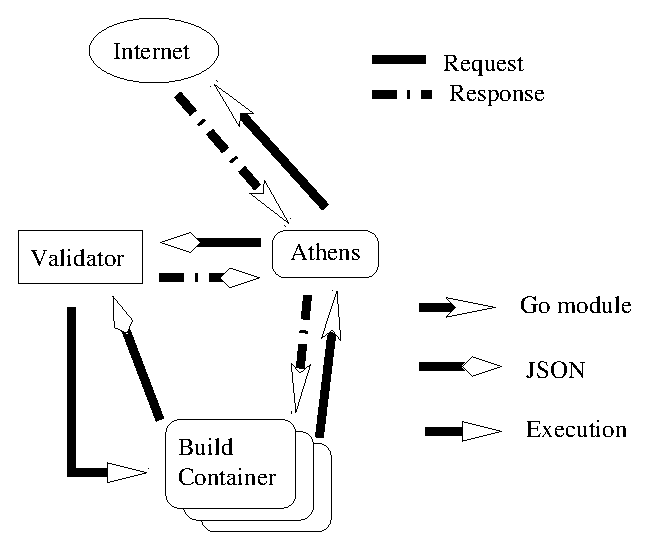
\includegraphics{architecture.eps}
\end{figure}


The validator considers all module/version tuples as valid. If the
specific module/version tuple has not been seen before, a build of
that is started\footnote{Technically, placed in a build queue}. The
validator limits builds to at most five concurrent ones, this is to
preserve some responsitivity on the test machine. It is possible to
increase the build parallelism by having more ``build workers''. The
number of build workers is set at compile time.

The custom build environment then reports back some general statistics
(did ``go mod download'' work, could we list all targets in the
downloaded code, did all builds succeed, did all tests succeed, how
many build/test targets, did go vet pass\footnote{This is a new test
  for this report}, and (on failure) what build/test targets
failed). The build environment is set up to use the Athens instance as
its GOPROXY, making it much easier to get a wide spectrum of code
scanned, as all transitive dependencies from the seed modules end up
being processed.

The validator periodically writes its current data set to disk. There
is also a web endpoint that triggers a save when accessed. The
validator will only create a new save file if there's been any
changes\footnote{Note, a ``change'' really means ``there has been
  build results reported'', in practice this is enough in the early
  stages of data gathering.}  since the last save.

To seed the scan, a few packages were manually started within the
build container, using the same environment as that set up by the
validator. For more details, see the section on seed packages.

The source code for the tabulator, the validation web-hook framework
and the build instrumentation can be found at
https://github.com/vatine/gochecker/ .


\subsection{Methodology changes for the latest report}

\subsubsection{Downloads}

Due to various changes in how Go modules are fetched, the wrapper has
been intrsumented to report ``module that can be downloaded, but has
one or more immediate missing dependencies'' as ``download succeeded,
build error'', whereas in previous versions that may have been
reported as a download error.

\subsubsection{Data cleaning}

The latest report also has a ``data cleaning'' component, that deletes
names tha can definitely not be module names (bare host names, github
users or organisations, golang.org/x and a few others, specific
details will be in source code). Only module-version tuples flagged as
``download failed'' are eligible for being cleaned from the data set.


\section{Recommendations based on this research}

The conclusions in this section remain mostly unchanged from the first
iteration of this line of investigation.

\subsection{Modules}

By all means make your code into a module, it improves the situation
for any user of your code, and may also make your life easier
(although in some cases it may make it harder).

At least a few of the build errors seen can be directly traced to not
having go modules enabled, so as a general recommendation, it is
probably something that should be done.

\subsection{Renaming}
It is recommended to never rename a Go module. If you want it available
under a new name, consider the new name a ``new module'' and leave
releases up to the point in time where the changed version still
available under the old name. If necessary, archive the repository, so
that no further accidental modifications are possible. Probably after
leaving a link in a README pointing to the new location.

Otherwise, the renaming has suddenly broken previously-fine
packages. If nothing else, the name change is putting a burden on any
user of your library and should ideally be followed up with a pull
request\footnote{The use of github.com as a platform is quite
  prevalent, other version control systems have different names for
  ``this is a unit of change''.} to bring users of the library back to
a building state.

Note that prior to the introduction of the module system, renames were
(to some extent) transparent to code, which is probably why the
practise continues even in a ``we should all be using modules now''
world.

The main reason I am recommending ``don't rename'' is that the name of
a module is (part of) its unique identifier, and with that changing,
on some level it is no longer ``the same module''. If nothing else, it
now has another name.

\subsection{Testing}

It is recommended to have pull requests checked against all (or at
least all relevant) test targets as part of the review
process. Ideally, this should be done by automation, posting status
back to the project.

It is strongly recommended to not cut a release if there are any
failing unit tests.

It may also be useful having periodic (daily? weekly? monthly?) builds
running with the latest toolchain, even if that's not the primary
concern while developing. Sooner or later, your library will end up in
a newer toolchain. And while the Go backwards compatibility guarantees
are pretty good, this report shows that sometimes things change subtly.


\section{The numbers}

Here are some numbers distilled from the investigation. For the
breakdown on failing build/test cases, the mean has only been done for
module/versions with at least one failure. The number of packages with
download problems is over-reported, as it includes: packages with a
name that differs from the requested in their go.mod, packages with a
version number that doesn't parse, and packages that simply do not
exist at this point in time.

\begin{table}[ht]
\caption{Build target statistics}
\label{table:build}
\begin{tabular}{|l|r|}
 \hline
  Packages processed & 4326 \\
  Packages failed to download & 1535 \\
  No build failures & 2604 (60.194175\%) \\
  No vet failures & 1789 (41.354600\%) \\
  No fmt failures & 4326 (100.000000\%) \\
  No test targets & 748 (17.290800\%) \\
 \hline
  Mean build targets (all modules)& 32.659270 \\
  stddev & 153.801803 \\
  Median build targets & 2 \\
  75th percentile \# of build targets & 10 \\
  90th percentile \# of build targets & 49 \\
  95th percentile \# of build targets & 185 \\
  99th percentile \# of build targets & 412 \\
  Max \# of build targets & 2674 \\
 \hline
  Mean build targets (at least one buildable)& 35.276904 \\
  stddev & 159.558912 \\
 \hline
  Mean failed build targets (all modules)& 20.178687 \\
  stddev & 147.212632 \\
 \hline
  Mean failed build targets (at least one failed)& 58.040559 \\
  stddev & 245.280695 \\
 \hline
  Mean failed vet targets (all modules)& 22.294267 \\
  stddev & 147.749693 \\
 \hline
  Mean failed vet targets (at least one failed)& 43.522112 \\
  stddev & 204.207778 \\
 \hline
\end{tabular}
\end{table}

\begin{table}[ht]
\caption{Test target statistics}
\label{table:test}
\begin{tabular}{|l|r|}
 \hline
  Packages seen & 4326 \\
  No test failures & 2165 (50.046232\%) \\
  No test failures (with tests) & 1417 (39.603130\%) \\
  No build failures, but test failures & 670 (15.487748\%) \\
  No tests & 748 (17.290800\%) \\
 \hline
  Mean failed test targets for passed builds (all) & 1.356716 \\
  stddev & 1.128344 \\
 \hline
  Mean failed test targets for passed builds (at least one fail) & 1.356716 \\
  stddev & 1.128344 \\
 \hline
  Mean failed test targets, all packages& 7.093012 \\
  stddev & 14.636305 \\
 \hline
  Mean failed test targets, packages with at least one test failure& 7.888832 \\
  stddev & 15.231140 \\
 \hline
\end{tabular}
\end{table}

\begin{table}[ht]
\caption{Most versions per module that  download}
\label{table:versions}
\begin{tabular}{|l|r|}
\hline
 golang.org/x/sys & 169 \\
 golang.org/x/tools & 139 \\
 google.golang.org/genproto & 130 \\
 golang.org/x/net & 109 \\
 google.golang.org/api & 62 \\
 cloud.google.com/go & 47 \\
 golang.org/x/crypto & 42 \\
 github.com/Azure/go-autorest/autorest & 31 \\
 google.golang.org/grpc & 28 \\
 github.com/prometheus/common & 27 \\
\hline
\end{tabular}
\end{table}
\begin{table}[ht]
\caption{Most versions per module that fail to download}
\label{table:failversions}
\begin{tabular}{|l|r|}
\hline
 github.com/hashicorp/consul & 72 \\
 golang.org/x/tools & 54 \\
 github.com/Azure/go-autorest & 53 \\
 google.golang.org/grpc & 40 \\
 github.com/hashicorp/vault & 37 \\
 contrib.go.opencensus.io/exporter & 36 \\
 golang.org/x/crypto & 34 \\
 github.com/aws/aws-sdk-go & 33 \\
 golang.org/x/exp & 21 \\
 github.com/Azure/go-autorest/autorest & 21 \\
\hline
\end{tabular}
\end{table}


\subsection{Download problems}

The number of packages that failed to download has increased
dramatically from the previous report, now standing at 1535, up from
last report's 340. Some of this is due to redirection domain names no
longer existing, some of this is down to more aggressive ``there are
missing dependencies'' in the toolchain.

Some of the download problems may stem from automatic ``try fetching a
shortened module path''\footnote{an example would be starting with
  ``golang.org/x/module@vx.y.z'', when that fails re-try with
  ``golang.org/x@vx.y.z'', and finally ``golang.org@vx.y.z'', if you
  start with an import that is in a deep-ish path within a module that
  has a problem, this can cause multiple counts of download failures}.

At this point, the clean-up is somewhat ad-hoc, addressing issues that
have been manually spotted and (in a limited number of cases) extended
to cover more incorrect import paths following the same pattern.

\subsection{Building}

Of the downloaded 4326 packages, 2604 (60.19\%) had no build
failures. This is a dramatic drop from the previous report, where 4598
out of 5108 (90.02\%) had no build failures.

At the time of writing this, no exhaustive investigation to find common
sources of these has been done.

Like in previous reports, this time we see a very skewed distribution
of build targets, with a few modules having may build targets
massively skewing the distribution. The median number of build targets
in a module is 2, the 75th percentile is 10, and the maximum number of
build targets seen is 2674. These numbers are lower than in the last
report, but MAY be influenced by multiple modules having downloaded
but in such a way that no target introspection can succeed.

\subsection{Go vet checks}

The Go toolchain has a built-in tool for reporting on possible
problems with the code that aren't wrong, per se, but have been found
to be problematic. This is invokable as {\tt go vet {\it target}}
and exits with a ``failure''\footnote{non-zero, in the case of unix}
status if there was anything to report.

This check has NOT been performed for packages that downloaded
successfully, but had one or more missing dependedncies.

\subsection{Go fmt checks}

New for this report is checking downloaded packages for conformance to
the {\tt go fmt} tool. This check has NOT been done for packages with
one or more missing dependencies, so may be artificially inflated.


\subsection{Tests}

The Go toolchain has a built-in test framework (accessible by running
{\tt go test {\it target}}) and it exits with a failure if any
specific test for that target fails. This does not give us a ``number
of failed tests'' (multiple failing tests within a single testable
target will only be counted once), but does give us an indication of
to what extent things are released (and used) with failing tests.

This round of testing was done with the Go 1.16.3 release. It started
with Go 1.16.0, then was re-done with 1.16.3 when there were what
seemed like anomalies in the data. This turns out to be a combination
of more aggressive ``nope, there are missing dependencies, so this
download has now failed'' and a few other small things.


Of the test failure numbers, the two that are probably most
interesting to compare are the ``no test failures (with tests)'' (that
is, at least one test target, and all tests pass), which distressingly
has dropped dramatically from the previous report (now 39.6\%,
previously 55.25\%) and the ``No build failures, but at least one
failing test'' (15.49\%, down from 30.38\%). Now, there's no further
breakdown than that, but we can at least assume that ``build failure''
would at least potentially cause ``test failure'' and there's a decent
margin between the two.

Slighly discouraging, 17.29\% of the packages had no test targets at
all, this is a combination both of ``a higher number of packages had
no tests'' (728 in the last report, 748 in this report) and ``a larger
proportion of modules failed to download''.

\section{Investigation of (some) download errors}

A module at a specific version is counted as ``has download error'' if
both a {\tt go mod download ...} and a {\tt go get ...} fail. This is
usually down to a discrepancy between the path of the module as
requested, and the name in the go.mod file. Not all errors have been
exhaustively investigated, but a few are investigated in more detail
below.

It is also counted as a ``download error'' if it is not possible to
list the contents of the package, this is a rather generous definition
of ``download error'', but from the background of ``go proxy for a
walled garden, wanting some assurance of what comes in'', it makes
some level of sense.

The 192.168.1.2:3000 you will see in a few error messages is simply
the Athens proxy that is part of the test environment.


\subsection{cloud.google.com/go/bigquery@v1.0.0}

This module/version combo fails with the following error:
\begin{verbatim}
go: downloading cloud.google.com/go/bigquery v1.0.0
go: downloading cloud.google.com/go v0.44.1
go: downloading cloud.google.com/go/bigquery v1.18.0
go: downloading cloud.google.com/go v0.82.0
cloud.google.com/go/bigquery: ambiguous import: found package cloud.google.com/go/bigquery in multiple modules:
	cloud.google.com/go v0.44.1 (/go/pkg/mod/cloud.google.com/go@v0.44.1/bigquery)
	cloud.google.com/go/bigquery v1.0.0 (/go/pkg/mod/cloud.google.com/go/bigquery@v1.0.0)
\end{verbatim}

This seems to be a new behaviour of the tool chain from 1.16 onwards.

\subsection{cloud.google.com/go/pubsub@v1.0.1-beta.ordered.keys}

This module/version fails with the following error:
\begin{verbatim}
go: downloading cloud.google.com/go/pubsub v1.0.1-beta.ordered.keys
go get: cloud.google.com/go/pubsub@v1.0.1-beta.ordered.keys requires cloud.google.com/go/pubsub@v1.0.1, not cloud.google.com/go/pubsub@v1.0.1-beta.ordered.keys
\end{verbatim}

This seems to be some weird circular reference, that I have not investigated deeper.

\section{cloud.google.com/go@v0.26.0}

Another case of ``transitive dependencies failing to download'' that the existing tooling doesn't take into account.

\begin{verbatim}
go: downloading cloud.google.com/go v0.23.0
go: downloading github.com/golang/protobuf v1.5.2
go: downloading github.com/googleapis/gax-go v1.0.3
go: downloading go.opencensus.io v0.23.0
go: downloading golang.org/x/net v0.0.0-20210521195947-fe42d452be8f
go: downloading golang.org/x/oauth2 v0.0.0-20210514164344-f6687ab2804c
go: downloading golang.org/x/sync v0.0.0-20210220032951-036812b2e83c
go: downloading google.golang.org/api v0.47.0
go: downloading google.golang.org/genproto v0.0.0-20210521181308-5ccab8a35a9a
go: downloading google.golang.org/grpc v1.38.0
go: downloading google.golang.org/api v0.0.0-20180910000450-7ca32eb868bf
go: downloading github.com/googleapis/gax-go v1.0.0
go: downloading google.golang.org/genproto v0.0.0-20180831171423-11092d34479b
go: downloading google.golang.org/grpc v1.14.0
go: downloading go.opencensus.io v0.18.0
go: downloading google.golang.org/appengine v1.6.7
go: downloading google.golang.org/protobuf v1.26.0
go: downloading golang.org/x/sys v0.0.0-20210514084401-e8d321eab015
go: downloading golang.org/x/sys v0.0.0-20210521203332-0cec03c779c1
go: downloading golang.org/x/text v0.3.6
go: downloading contrib.go.opencensus.io/exporter/stackdriver v0.13.6
go: downloading contrib.go.opencensus.io/exporter/stackdriver v0.6.0
cloud.google.com/go tested by
	cloud.google.com/go.test imports
	golang.org/x/oauth2/google: cannot find module providing package golang.org/x/oauth2/google
cloud.google.com/go tested by
	cloud.google.com/go.test imports
	google.golang.org/api/option imports
	golang.org/x/oauth2: cannot find module providing package golang.org/x/oauth2
cloud.google.com/go tested by
	cloud.google.com/go.test imports
	cloud.google.com/go/datastore imports
	google.golang.org/api/transport/grpc imports
	google.golang.org/grpc/credentials/oauth imports
	golang.org/x/oauth2/jwt: cannot find module providing package golang.org/x/oauth2/jwt
\end{verbatim}


\subsection{code.gitea.io/sdk@v0.14.0}

This simply fails with a 404 error. Looking at the versions listed on
pkg.go.dev, v0.14.0 is not displayed. The package is not
module-enabled, but the documentation has a longer import path ({\tt
  import "code.gitea.io/sdk/gitea"}) listed.

This MAY be a case of a shortened URL, as there are also entries for
the longer path.

\subsection{contrib.go.opencensus.io/exporter/ocagent@v0.4.6}

This is failing due to a non-existing dependency, but in a fashion that the existing toolchain doesn't recognise as such.

\begin{verbatim}
go: contrib.go.opencensus.io/exporter/ocagent@v0.4.6 requires
	github.com/census-instrumentation/opencensus-proto@v0.1.0-0.20181214143942-ba49f56771b8: reading http://192.168.1.2:3000/github.com/census-instrumentation/opencensus-proto/@v/v0.1.0-0.20181214143942-ba49f56771b8.mod: 404 Not Found
\end{verbatim}


\section{Investigation of (some) build errors}

There are some packages that do not work to download with ``go mod
download'', this seems to be down to structural problems with the
repositories, like ``at higher than v1, but not under a v2 (or later)
path prefix''. Observing that this is a possible source of ``fewer
transitive dependencies'' as well as ``possibly false failed
download'' numbers, the build environment has been changed to first
try a ``go mod download'', and if that fails, a ``go get'' at the same
version.

Some packages fail because the path declared in their go.mod does not
correspond to the path their dependencies have
declared\footnote{Changing ``full name'' of a Go module is
  problematic, as that effectively changes the ``unique identifier''}.

In some cases, an erroneous version number has snuck in, causing
problems downloading the package\footnote{This seems prevalent for
  packages listing dependencies under k8s.io, for some reason}. One
possibility may be that the go.mod file using local rewrites for
dependencies. These work for the ``root'' package, but do not work
during a transitive build. Another possibility is an automatic attempt
to convert a godeps dependency file to a go.mod.

\subsection{cloud.google.com/go/bigquery@v1.7.0}

This is a simple build error, but interesting in that it shoudl be
catchable with checks during code review. It could be that it is for
``this is how the code WILL look'', or other code having changed since
merge.

\begin{verbatim}
# cloud.google.com/go/bigquery/reservation/apiv1beta1
/go/pkg/mod/cloud.google.com/go/bigquery@v1.7.0/reservation/apiv1beta1/reservation_client.go:728:111: req.GetBiReservation undefined (type *reservation.UpdateBiReservationRequest has no field or method GetBiReservation)
    Build of cloud.google.com/go/bigquery/reservation/apiv1beta1 failed
\end{verbatim}


\subsection{cloud.google.com/go/pubsub@v1.0.0}

This error is because the go.sum file for this specific version of the
module genuinely does not contain any data for
golang.org/x/time/rate. On the flip side, there is no go.mod file for
golang.org/x/time/rate, but there is one for golang.org/x/time, so
there's something a bit weird happening here.

Not surprising, we are seeing two build targets failing on the same
thing, both included for completeness sake.

\begin{verbatim}
DEBUG:root:  Building go target cloud.google.com/go/pubsub/loadtest
DEBUG:root:Running go build cloud.google.com/go/pubsub/loadtest
/go/pkg/mod/cloud.google.com/go/pubsub@v1.0.0/loadtest/loadtest.go:35:2: missing go.sum entry for module providing package golang.org/x/time/rate (imported by cloud.google.com/go/pubsub/loadtest); to add:
	go get cloud.google.com/go/pubsub/loadtest@v1.0.0
DEBUG:root:    Build of cloud.google.com/go/pubsub/loadtest failed
DEBUG:root:Running go vet cloud.google.com/go/pubsub/loadtest
/go/pkg/mod/cloud.google.com/go/pubsub@v1.0.0/loadtest/loadtest.go:35:2: missing go.sum entry for module providing package golang.org/x/time/rate (imported by cloud.google.com/go/pubsub/loadtest); to add:
	go get cloud.google.com/go/pubsub/loadtest@v1.0.0
...
DEBUG:root:  Building go target cloud.google.com/go/pubsub/loadtest/cmd
DEBUG:root:Running go build cloud.google.com/go/pubsub/loadtest/cmd
/go/pkg/mod/cloud.google.com/go/pubsub@v1.0.0/loadtest/loadtest.go:35:2: missing go.sum entry for module providing package golang.org/x/time/rate (imported by cloud.google.com/go/pubsub/loadtest); to add:
	go get cloud.google.com/go/pubsub/loadtest@v1.0.0
DEBUG:root:    Build of cloud.google.com/go/pubsub/loadtest/cmd failed
DEBUG:root:Running go vet cloud.google.com/go/pubsub/loadtest/cmd
/go/pkg/mod/cloud.google.com/go/pubsub@v1.0.0/loadtest/loadtest.go:35:2: missing go.sum entry for module providing package golang.org/x/time/rate (imported by cloud.google.com/go/pubsub/loadtest); to add:
	go get cloud.google.com/go/pubsub/loadtest@v1.0.0
\end{verbatim}

\subsection{github.com/DATA-DOG/go-sqlmock@v1.4.1}
\begin{verbatim}
Running go vet github.com/DATA-DOG/go-sqlmock/examples/orders
/go/pkg/mod/github.com/!d!a!t!a-!d!o!g/go-sqlmock@v1.4.1/examples/orders/orders.go:8:2: no required module provides package github.com/kisielk/sqlstruct; to add it:
	go get github.com/kisielk/sqlstruct

\end{verbatim}

This is due to a go.mod file that does NOT contain any of the
dependencies. This release also does not have a go.sum file, meaning
that repeatability in build is not guaranteed (actually, pretty much
the opposite).



\section{Investigation of (some) test errors}

As a general comment, it is a bit surprising that tagged releases have
test errors at all, indicating that there's improvements to make
around release processes.

In some cases, this is because the tooling
has changed what constitutes a ``passing'' test (over time, some ``go
vet'' warnings have become errors when they occur during a run of {\tt
  go test}) and the CI pipeline is running with ``not the most recent
release'', a situation that is totally understandable.

There's also the case of a release
that was made before the most current, which for obvious reasons will
not have had a CI run against a version released after
itself\footnote{But, if you can provide a CI system that will reliably
  test against compiler versions released in the future from the time
  the test is run, the author is interested in testing them...}

For practical reasons, the testing has not been re-run with prior
versions of the Go toolchain to find where things may have started
acting up, even in the manual investigations that follow.

We will now look closer at a few packages. I have explicitly excluded
packages that have build failures from closer inspection, as the test
may well be because of one (or more) build failures due to missing
dependencies.

The methodology for choosing packages is (approximately) looking
through the emitted latest data file, in whatever order the JSON
marshalling places things, investigate more closely what the test
warnings are, until it is no longer fun to dig anymore.

\subsection{cloud.google.com/go/bigquery@v1.0.1}
\begin{verbatim}
# cloud.google.com/go/bigquery/datatransfer/apiv1 [cloud.google.com/go/bigquery/datatransfer/apiv1.test]
/go/pkg/mod/cloud.google.com/go/bigquery@v1.0.1/datatransfer/apiv1/mock_test.go:428:3: unknown field 'DestinationDatasetId' in struct literal of type datatransfer.TransferConfig
/go/pkg/mod/cloud.google.com/go/bigquery@v1.0.1/datatransfer/apiv1/mock_test.go:507:3: unknown field 'DestinationDatasetId' in struct literal of type datatransfer.TransferConfig
/go/pkg/mod/cloud.google.com/go/bigquery@v1.0.1/datatransfer/apiv1/mock_test.go:638:3: unknown field 'DestinationDatasetId' in struct literal of type datatransfer.TransferConfig
/go/pkg/mod/cloud.google.com/go/bigquery@v1.0.1/datatransfer/apiv1/mock_test.go:845:3: unknown field 'DestinationDatasetId' in struct literal of type datatransfer.TransferRun
FAIL	cloud.google.com/go/bigquery/datatransfer/apiv1 [build failed]
FAIL
\end{verbatim}

This seems to be an outright mistake in the code. Looking at the
datatransfer.TransferConfig type definition, I can't find any instance
at which it has a member named that. The closest is that there's a
{\tt Destination} struct member typed as a package-internal interface,
with an exported type named  {\tt TransferConfig\_DestinationDatasetId}
that, in turn, has a {\tt DestinationDatasetId} struct member.

\subsection{contrib.go.opencensus.io/exporter/ocagent@v0.4.12}
\begin{verbatim}
# contrib.go.opencensus.io/exporter/ocagent [contrib.go.opencensus.io/exporter/ocagent.test]
/go/pkg/mod/contrib.go.opencensus.io/exporter/ocagent@v0.4.12/viewdata_to_metrics_test.go:51:45: cannot use ma (type *metricsAgent) as type "github.com/census-instrumentation/opencensus-proto/gen-go/agent/metrics/v1".MetricsServiceServer in argument to "github.com/census-instrumentation/opencensus-proto/gen-go/agent/metrics/v1".RegisterMetricsServiceServer:
	*metricsAgent does not implement "github.com/census-instrumentation/opencensus-proto/gen-go/agent/metrics/v1".MetricsServiceServer (missing "github.com/census-instrumentation/opencensus-proto/gen-go/agent/metrics/v1".mustEmbedUnimplementedMetricsServiceServer method)
FAIL	contrib.go.opencensus.io/exporter/ocagent [build failed]
FAIL
\end{verbatim}

\subsection{github.com/JamesClonk/vultr@v0.0.0-20210225162646-a13a15c46955}
\begin{verbatim}
# github.com/JamesClonk/vultr/lib
/go/pkg/mod/github.com/!james!clonk/vultr@v0.0.0-20210225162646-a13a15c46955/lib/account_info_test.go:7:2: missing go.sum entry for module providing package github.com/stretchr/testify/assert (imported by github.com/JamesClonk/vultr/lib); to add:
	go get -t github.com/JamesClonk/vultr/lib@v0.0.0-20210225162646-a13a15c46955
FAIL	github.com/JamesClonk/vultr/lib [setup failed]
FAIL

\end{verbatim}

I am not at all sure why we're seeing this error message. At the 1.3.0
version, there is a go.mod for {\tt github.com/stretchr/testify}, and
there is none for the {\tt assert} subdirectory.

\subsection{github.com/Rican7/retry@v0.1.0}
\begin{verbatim}
# github.com/Rican7/retry
vet: /go/pkg/mod/github.com/!rican7/retry@v0.1.0/retry_test.go:143:6: logFile declared but not used
FAIL	github.com/Rican7/retry [build failed]
FAIL
\end{verbatim}

This is a pretty classic Go error message. There is an unused
variable, which (for good or bad) is a compile error.

In this specific case, it is in an example, but it looks like the test
file has actual tests in addition to the examples.

\subsection{github.com/aokoli/goutils@v1.0.1}
\begin{verbatim}
# github.com/aokoli/goutils
/go/pkg/mod/github.com/aokoli/goutils@v1.0.1/randomstringutils.go:118:44: conversion from int to string yields a string of one rune, not a string of digits (did you mean fmt.Sprint(x)?)
FAIL	github.com/aokoli/goutils [build failed]
FAIL
\end{verbatim}

This is one of those Go vet checks that have been promoted to ``flag
as a failure during tests''. There are a few more of those and as a
general rule, some code from ``before this was enabled'' may still
have it.

\subsection{github.com/appc/spec@v0.8.11}
\begin{verbatim}
/go/pkg/mod/github.com/appc/spec@v0.8.11/schema/types/semver.go:20:2: no required module provides package github.com/coreos/go-semver/semver; to add it:
	go get github.com/coreos/go-semver/semver
/go/pkg/mod/github.com/appc/spec@v0.8.11/schema/types/resource/quantity.go:28:2: no required module provides package github.com/spf13/pflag; to add it:
	go get github.com/spf13/pflag
/go/pkg/mod/github.com/appc/spec@v0.8.11/schema/image.go:25:2: no required module provides package go4.org/errorutil; to add it:
	go get go4.org/errorutil
/go/pkg/mod/github.com/appc/spec@v0.8.11/schema/types/resource/amount.go:23:2: no required module provides package gopkg.in/inf.v0; to add it:
	go get gopkg.in/inf.v0
\end{verbatim}


This is a pre-module package, failing to build in many ways. This
seems to be the root of the test failure in this case.


\section{Seed packages}

This is the list of every seed package. 

This time, no exhaustive manual ``try each of the 718 failed packages
to see why'' has been done, leaving (potentially) interesting findings
by the wayside.

\begin{table}[ht]
  \caption{Seed modules and versions}
  \label{table:seed}
  \begin{itemize}
  \item github.com/containerd/containerd v1.3.6
  \item helm.sh/helm/v3 v3.3.4
  \item github.com/miekg/dns v1.1.29


  \end{itemize}
\end{table}


\end{document}
